\documentclass[11pt]{article}
\usepackage[margin=1in]{geometry}
\usepackage{amsmath,amssymb,amsthm,mathtools}
\usepackage{graphicx}
\usepackage[hidelinks]{hyperref}
\usepackage{microtype}

\newtheorem{theorem}{Theorem}
\newtheorem{lemma}[theorem]{Lemma}
\newtheorem{proposition}[theorem]{Proposition}
\newtheorem{corollary}[theorem]{Corollary}
\newcommand{\BH}{\mathbb B(\mathcal H)}
\newcommand{\G}{\mathbf G}
\newcommand{\A}{\mathbf A}

\title{The Multivariate Operator Alzer Inequality\\
via a L\"owner-Monotone Complement Path}
\author{Candidate full solution to the open problem in arXiv:1806.10806}
\date{17 August 2026}

\begin{document}
\maketitle

\begin{center}
\fbox{\parbox{0.9\linewidth}{\textbf{Status.} Candidate full solution, likely valid pending expert review.  The proof covers arbitrary (not necessarily commuting) positive operators and also gives the equality case.}}
\end{center}

\section{Source problem}

Morassaei and Mirzapour ask on pages 5--6 of \cite{MM} whether, for
$0<A_j\leq \tfrac12 I$, the recursively ordered geometric mean satisfies
\begin{equation}\label{eq:source}
   \A_n'-\G_n'\ \leq\ \A_n-\G_n.
\end{equation}
Here $A_j'=I-A_j$, $\A_n=n^{-1}\sum_j A_j$, and primes on the means
mean that they are evaluated at $(A_1',\ldots,A_n')$.  The source's
geometric mean is
\begin{align*}
 X\#_\alpha Y
   &=X^{1/2}(X^{-1/2}YX^{-1/2})^\alpha X^{1/2},\\
 \G_1(A_1)&=A_1,\qquad
 \G_m(A_1,\ldots,A_m)
   =A_1\#_{(m-1)/m}\G_{m-1}(A_2,\ldots,A_m).
\end{align*}
The two images below reproduce the complete statement.

\begin{center}
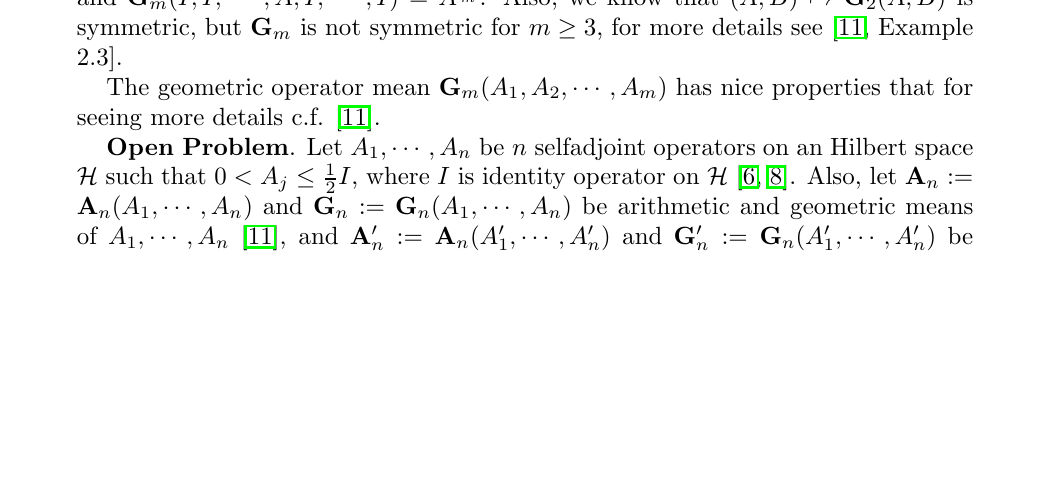
\includegraphics[width=\linewidth]{figures/open_problem_crop_page5.png}

\smallskip
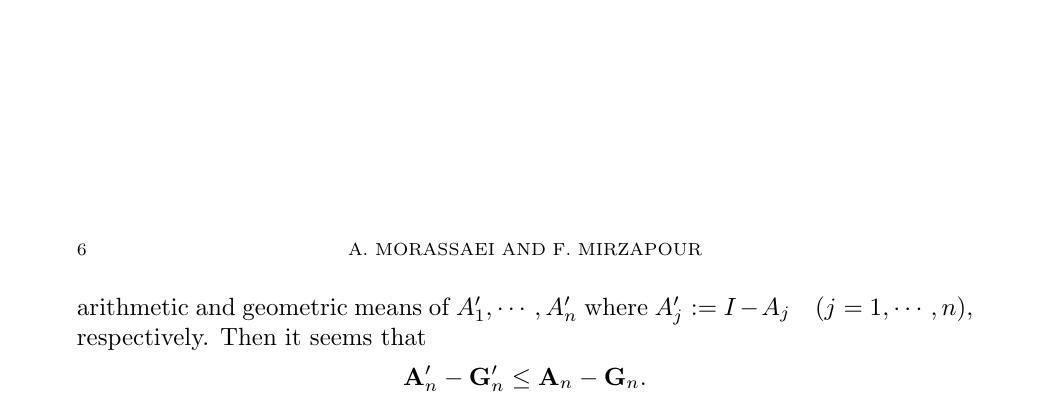
\includegraphics[width=\linewidth]{figures/open_problem_crop_page6.png}
\end{center}

\section{Proof intuition}

Join each $A_j$ to its complement by
\[
  A_j(t)=A_j+t(I-2A_j),\qquad 0\leq t\leq1.
\]
All directions $I-2A_j$ are positive, and every path passes through the
same point $I/2$ at $t=1/2$.  Joint monotonicity and direct-sum covariance of
the recursive geometric mean imply something stronger than ordinary
monotonicity: every scalar quadratic form of
$F(t)=\G_n(A_1(t),\ldots,A_n(t))$ is an operator-monotone scalar function of
$t$.  L\"owner's integral representation then says that its secant over
$[0,1]$ dominates its derivative at $1/2$.  At the common diagonal point,
the derivative of $\G_n$ is exactly the arithmetic average of the input
directions.  This turns the secant inequality into \eqref{eq:source} after
one rearrangement.  A second-order expansion at the diagonal also yields
the equality characterization.

\section{Two one-variable lemmas}

\begin{lemma}[midpoint secant inequality]\label{lem:scalar}
Let $f:[0,\infty)\to[0,\infty)$ be operator monotone and continuous at
zero.  Then
\begin{equation}\label{eq:midpoint}
   f(1)-f(0)\ \geq\ f'(1/2).
\end{equation}
Equality holds only if $f$ is affine on $(0,\infty)$.
\end{lemma}

\begin{proof}
The L\"owner representation for a nonnegative operator-monotone function on
the positive half-line can be written
\[
 f(t)=a+bt+\int_{(0,\infty)}\frac{t}{t+\lambda}\,d\mu(\lambda),
 \qquad a,b\geq0,
\]
after absorbing harmless positive normalizing factors into the positive
measure; continuity at zero absorbs a possible zero atom into $a$.
For the nonlinear kernel $k_\lambda(t)=t/(t+\lambda)$,
\[
 k_\lambda(1)-k_\lambda(0)-k_\lambda'(1/2)
 =\frac{1}{1+\lambda}-\frac{\lambda}{(\lambda+1/2)^2}
 =\frac{1}{4(1+\lambda)(\lambda+1/2)^2}>0.
\]
The affine part gives equality.  Integration proves \eqref{eq:midpoint};
equality forces the representing measure to vanish.
\end{proof}

\begin{lemma}[positive multivariate paths become operator monotone]
\label{lem:path}
Let $M$ be a positive operator map of $n$ positive variables which is
jointly monotone, respects orthogonal direct sums, and is unitarily
covariant.  If $P_j>0$ and $Q_j\geq0$, set
\[
   F(t)=M(P_1+tQ_1,\ldots,P_n+tQ_n),\qquad t\geq0.
\]
For every unit vector $u\in\mathcal H$, the scalar function
$f_u(t)=\langle F(t)u,u\rangle$ is nonnegative and operator monotone on
$[0,\infty)$.
\end{lemma}

\begin{proof}
Fix $r\geq1$ and positive matrices $S\leq T$ in $M_r$.  On
$\mathcal H\otimes\mathbb C^r$, put
\[
 \widehat F(S)=M(P_1\otimes I+Q_1\otimes S,\ldots,
                    P_n\otimes I+Q_n\otimes S).
\]
Joint monotonicity gives $\widehat F(S)\leq\widehat F(T)$.  If
$S=U\operatorname{diag}(s_1,\ldots,s_r)U^*$, direct-sum covariance and
unitary covariance give
\[
 \widehat F(S)=(I\otimes U)\operatorname{diag}
    (F(s_1),\ldots,F(s_r))(I\otimes U^*).
\]
Compressing by the isometry $V:\mathbb C^r\to\mathcal H\otimes\mathbb C^r$,
$Ve_k=u\otimes e_k$, yields
\[
   f_u(S)=V^*\widehat F(S)V\leq V^*\widehat F(T)V=f_u(T),
\]
where the outer occurrences of $f_u$ are ordinary scalar functional
calculus.  This holds for every $r$, hence $f_u$ is operator monotone.
\end{proof}

The recursive mean $\G_n$ satisfies the three hypotheses of
Lemma~\ref{lem:path}: weighted Kubo--Ando geometric means are monotone in
both variables, direct-sum preserving, and unitarily covariant, and these
properties pass through the recursion.

\section{Full solution}

\begin{lemma}[derivative at a scalar diagonal]\label{lem:derivative}
For selfadjoint $H_1,\ldots,H_n$ and $c>0$,
\[
 \left.\frac{d}{ds}\right|_{s=0}
 \G_n(cI+sH_1,\ldots,cI+sH_n)
 =\frac1n\sum_{j=1}^nH_j.
\]
\end{lemma}

\begin{proof}
At $(cI,cI)$ the first derivative of $X\#_\alpha Y$ in directions $(H,K)$
is $(1-\alpha)H+\alpha K$.  This follows immediately by expanding the
defining formula to first order.  Apply it to the recursion with
$\alpha=(n-1)/n$ and use induction.
\end{proof}

\begin{theorem}[multivariate operator Alzer inequality]\label{thm:main}
Let $n\geq2$ and let $A_1,\ldots,A_n\in\BH$ satisfy
$0<A_j\leq\tfrac12I$.  For the recursively ordered geometric mean in
\cite{MM},
\[
 \boxed{\quad \A_n'-\G_n'\ \leq\ \A_n-\G_n.\quad}
\]
No commutativity hypothesis is needed.  Equality holds if and only if
$A_1=\cdots=A_n$.
\end{theorem}

\begin{proof}
Put $Q_j=I-2A_j\geq0$ and
\[
 F(t)=\G_n(A_1+tQ_1,\ldots,A_n+tQ_n),\qquad t\geq0.
\]
Thus $F(0)=\G_n$, $F(1)=\G_n'$, and every input at $t=1/2$ equals
$I/2$.  Lemmas~\ref{lem:scalar} and \ref{lem:path}, applied to every unit
vector $u$, imply
\[
 \langle(F(1)-F(0)-F'(1/2))u,u\rangle\geq0.
\]
Lemma~\ref{lem:derivative} gives
\[
 F'(1/2)=\frac1n\sum_{j=1}^nQ_j=I-2\A_n.
\]
Consequently
\[
 \G_n'-\G_n\geq I-2\A_n,
\]
which is equivalent to
$I-\A_n-\G_n'\leq\A_n-\G_n$, namely the asserted inequality.

It remains to identify equality.  If equality holds, then equality holds
in Lemma~\ref{lem:scalar} for every scalarization, so
$F''(1/2)=0$.  We show that this forces all $Q_j$ to agree.  The
second-order expansion of a weighted geometric mean at a scalar diagonal is
\begin{equation}\label{eq:hessian}
 \left.(X\#_\alpha Y)''\right|_0
 =(1-\alpha)X''(0)+\alpha Y''(0)
 -\frac{\alpha(1-\alpha)}{c}\bigl(X'(0)-Y'(0)\bigr)^2,
\end{equation}
when $X(0)=Y(0)=cI$.  (Expand the defining formula to second order.)
Apply \eqref{eq:hessian} recursively at $c=1/2$.  If
$\overline Q_{2:n}=(n-1)^{-1}\sum_{j=2}^nQ_j$ and
$\alpha=(n-1)/n$, then
\[
 F_n''(1/2)=\alpha F_{n-1}''(1/2)
 -\frac{\alpha(1-\alpha)}{c}
       (Q_1-\overline Q_{2:n})^2.
\]
Inductively $F_{n-1}''(1/2)\leq0$.  A sum of two negative operators can
vanish only if both vanish.  Hence $Q_1=\overline Q_{2:n}$ and, recursively,
$Q_2=\cdots=Q_n$; therefore all $Q_j$, and all $A_j$, are equal.  The
converse is immediate because both arithmetic--geometric gaps then vanish.
\end{proof}

\section{Verification and scope}

The proof is dimension-free and does not use the arithmetic--geometric
upper bound.  Its essential review points are: (i) the amplification and
compression in Lemma~\ref{lem:path}; (ii) the standard positive-half-line
L\"owner representation; and (iii) the diagonal derivative in
Lemma~\ref{lem:derivative}.  The equality statement additionally uses only
the second-order identity \eqref{eq:hessian}.

Independent numerical tests in the accompanying code evaluated the exact
recursive mean by spectral functional calculus on large random collections
of real and complex positive matrices, including $n=3,4$ and dimensions
$2,3$, and a global/local optimization over real $2\times2$ triples.  No
negative eigenvalue beyond floating-point noise was found.  These tests are
sanity checks, not part of the proof.

The same argument proves a broader principle: any jointly monotone,
direct-sum preserving, unitarily covariant multivariate mean has the
complement inequality associated with its tangent weights at a scalar
diagonal.  The present theorem specializes those weights to $1/n$.

\section{Novelty check}

A bounded search on 17 August 2026 covered the run's cheap indexes and local
arXiv source corpus, exact-title/author searches for arXiv:1806.10806, and web
searches for ``multivariate operator Alzer inequality'', ``operator Ky Fan
type inequality'', and recursive/multivariate geometric-mean variants.  The
later paper \cite{HRM} cites the source and proves the arbitrary
noncommuting \emph{binary} Kubo--Ando-mean inequality, but it does not treat
the recursive $n$-variable problem.  Hansen \cite{Hansen} develops the
regularity and monotonicity framework for inductive multivariate geometric
means, but no complement inequality of the form above was located.  Thus
novelty confidence is moderate pending a specialist search.

\section{Human review recommendation}

Prioritize a check that the direct-sum calculation in
Lemma~\ref{lem:path} really identifies the compression with scalar functional
calculus for every matrix level.  Then check the normalization of the
L\"owner kernel in Lemma~\ref{lem:scalar} and the convention
$\G_m=A_1\#_{(m-1)/m}\G_{m-1}$.  The main inequality does not depend on the
equality-case Hessian calculation, so any issue confined to
\eqref{eq:hessian} would affect only the characterization of equality.

\begin{thebibliography}{9}
\bibitem{MM}
A. Morassaei and F. Mirzapour,
\emph{Alzer Inequality for Hilbert Spaces Operators},
arXiv:1806.10806 (2018).

\bibitem{HRM}
S. Habibzadeh, J. Rooin, and M. S. Moslehian,
\emph{Operator Ky Fan type inequalities},
arXiv:1811.00475 (2018), especially Theorem 3.1.

\bibitem{Hansen}
F. Hansen,
\emph{Regular operator mappings and multivariate geometric means},
arXiv:1403.3781 (2014).

\bibitem{Bhatia}
R. Bhatia,
\emph{Positive Definite Matrices}, Princeton University Press, 2007.
\end{thebibliography}

\end{document}
